\chapter{Evaluation}

In this chapter, we will evaluate our proposed planning model based on deep reinforcement learning built upon Transformer \ref{transformer} architecture utilizing Graph Attention Network \ref{graph-attention-network} and benchmark the performance against constructive heuristics and metaheuristics.

\section{Dataset}
The dataset used for training and evaluation was generated on the fly via a uniform probability distribution within a given range. The reason we decided to generate the data is that learning reinforcement policy requires a large amount of training data. Since it learns by interacting with the environment, we do not need labeled datasets and generating them seems as the best approach. Nevertheless, in further work, the model will require other kinds of distribution to simulate a real-world demand.

In real-world routing applications, the geographic coordinate system is typically used for specifying locations. However, our proposed model requires locations between $[0, 1]$ to achieve model convergence. The locations of depots and delivery nodes were generated via uniform distribution within a range of $[0, 1] \times [0, 1]$.

The data for the demand capacity of a delivery node is a discrete number $\{1, \cdots, 9\}$ chosen uniformly at random with assumption that the depot has a demand capacity of zero. 

Lastly, each location has assigned time windows that work as a soft constraint at which time a vehicle is supposed to visit the node. We generate different lengths of time windows based on the problem size (20, 50, 100). For the problem size of 20 nodes, the time window value occurs in a range of $\{0, \cdots, 10\}$ with the condition that the length of the time window is less than four. The problem size of 50 nodes has the upper bound set to 20 with a maximal length of 6 and the case of 100 nodes, the upper bound is 40 and the maximal window length is 9. Similarly, the start and end of a time window are generated with uniform distribution.

\section{Sample Solutions}
To better imagine the complexity and variability of solving \gls{vrptw}, in Figure \ref{fig:sample-20} and \ref{fig:sample-50} we illustrate a random solution predicted by our proposed deep learning model. On the left, we visualize the customer's time windows using Gantt diagram and on the right are shown the routes for each vehicle. Each color represents a vehicle which servers the customers represented by a node with a generated time window.

\begin{figure}[ht]
    \centering
    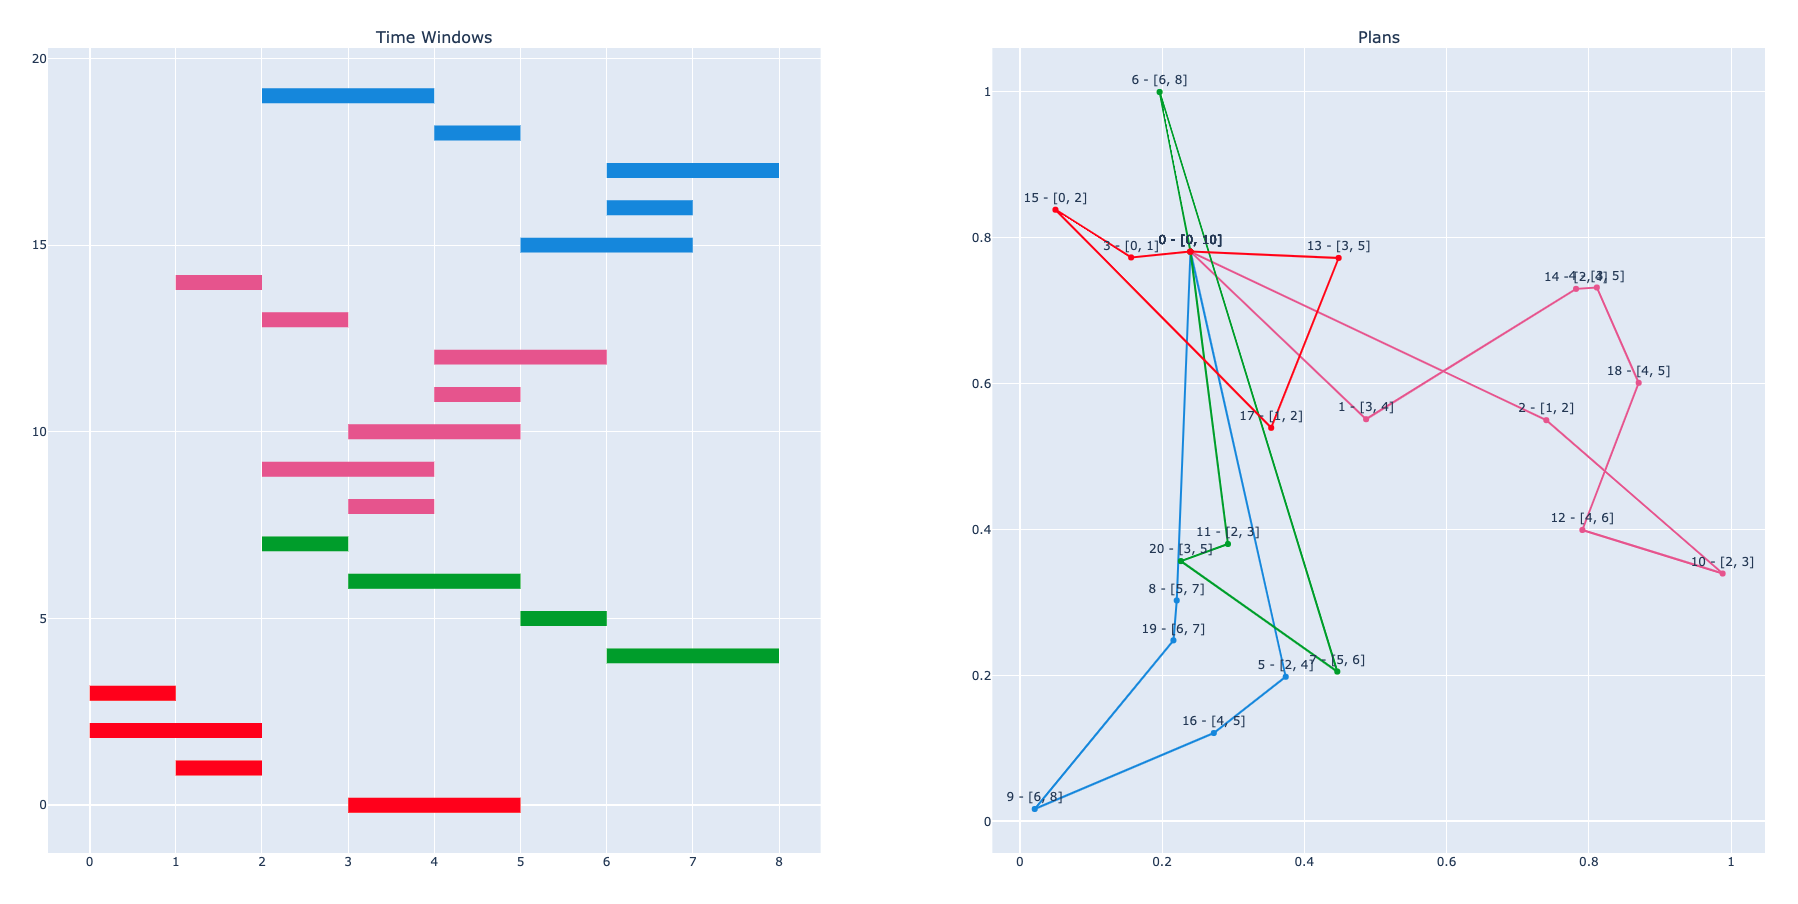
\includegraphics[width=1.0\textwidth]{resources/evaluation/sample-20.png}
    \caption{Sample solution of random \gls{vrptw} instance for problem size 20.}
    \label{fig:sample-20}
\end{figure}

The \gls{ai} model has to optimize the route path with focus to minimize the travelled distance, but simultaneously early and late arrivals should be avoided. Our model is able to solve \gls{vrptw} instance considers both distance and time window constrains. The windows are soft constrained, which results in a much larger combinatorial space of possible solutions than considering just hard constrained time windows. As illustrated on Figure \ref{fig:sample-50} the model sometimes sacrifices the time of a served customer in order to optimize the route distance and vice versa.

\begin{figure}[ht]
    \centering
    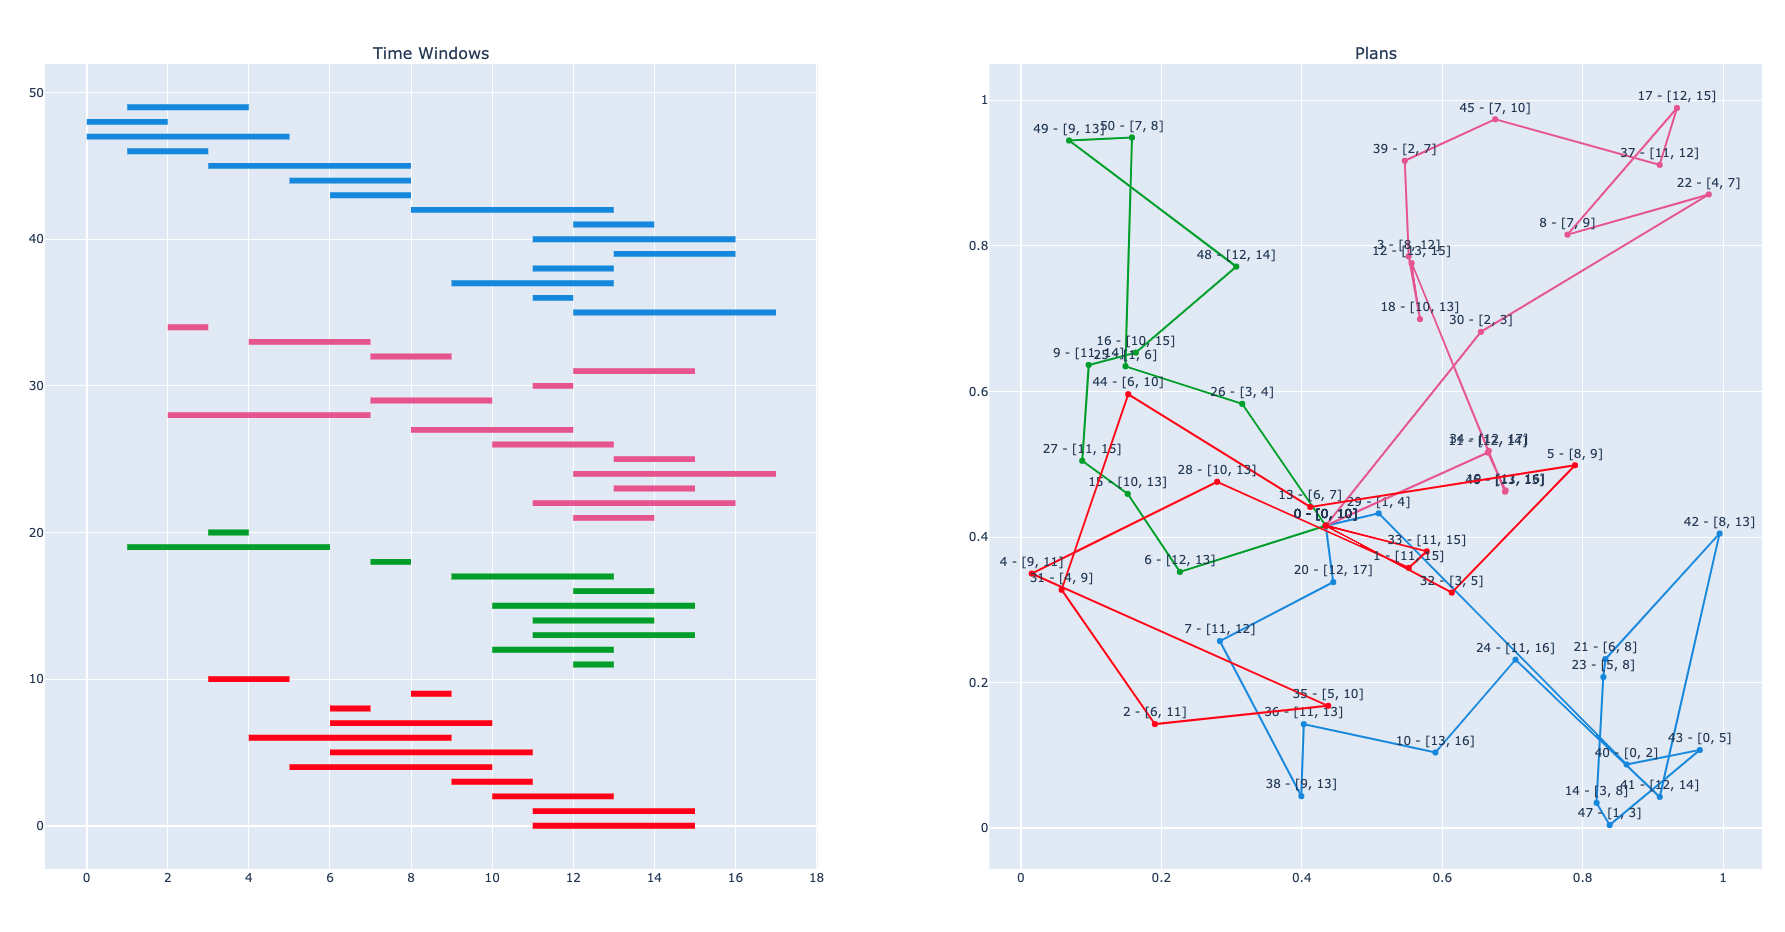
\includegraphics[width=1.0\textwidth]{resources/evaluation/sample-50.png}
    \caption{Sample solution of random \gls{vrptw} instance for problem size 50.}
    \label{fig:sample-50}
\end{figure}

The model has successfully learned the policy how to pick the next node to visit, the time windows are almost cascadingly sorted, and the routes are suboptimally optimized based on distance. However, it is clearly not an optimal solution, but it proves that the problem of vehicle routing with soft constrained time windows is possible to be solved with \gls{ml} and the research is on the right path to outperform regular metaheuristics. In the section \ref{benchmarking} we compare the model with our implemented constructive heuristics and metaheuristics

\section{Experiments}
\subsection{Time Windows}
The main goal of this thesis was to integrate the soft constraint of time windows to \gls{vrp} model introduced by Kool et al.\cite{attention-route}. The model is extended by our proposed cost function \ref{vrptw-cost} that penalizes early and late arrivals. The early arrival is not as crucial as delayed visit, so we have decided that the penalty for early arrival is always less than late visit $p_e < p_l$.

\begin{figure}[ht]
    \centering
    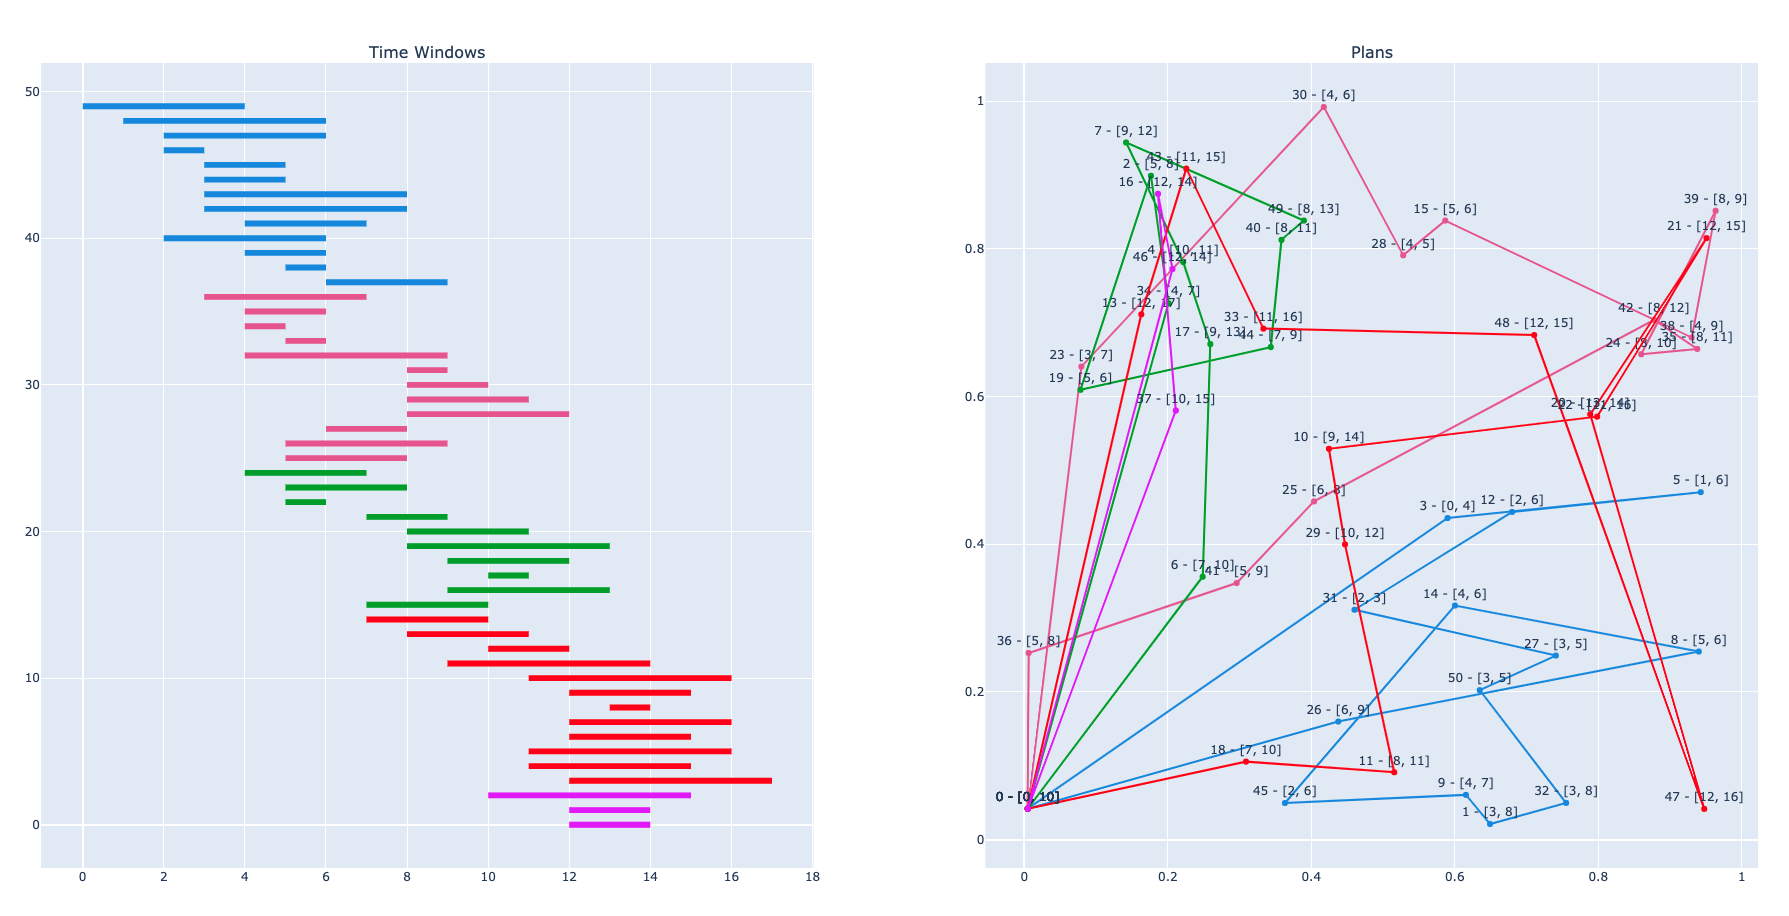
\includegraphics[width=1.0\textwidth]{resources/evaluation/tw-problem.png}
    \caption{Low penalty for early visit of node results in poor performance.}
    \label{fig:tw-problem}
\end{figure}

Finding a proper penalty values $p_e$ and $p_l$ for time windows is one of the most important steps because an incorrect penalty highly influences the model in choosing the next node to visit.

The Figure \ref{fig:tw-problem} illustrates how the performance is degraded by choosing an incorrect penalty value for early arrival $p_e$. If the early penalty is too low, the model will strictly focus on minimizing the late arrival and Gantt diagram of time windows looks like a plan for just a single vehicle.

We have empirically tested various kinds of penalties and updated them based on our observations. After the experiments, we have chosen $p_e = 0,25$ and $p_l  = 0,5$ which resulted in predicting a feasible plans with properly distributed time windows across the vehicles as shown in Figure \ref{fig:nice-tw}.

\begin{figure}[ht]
    \centering
    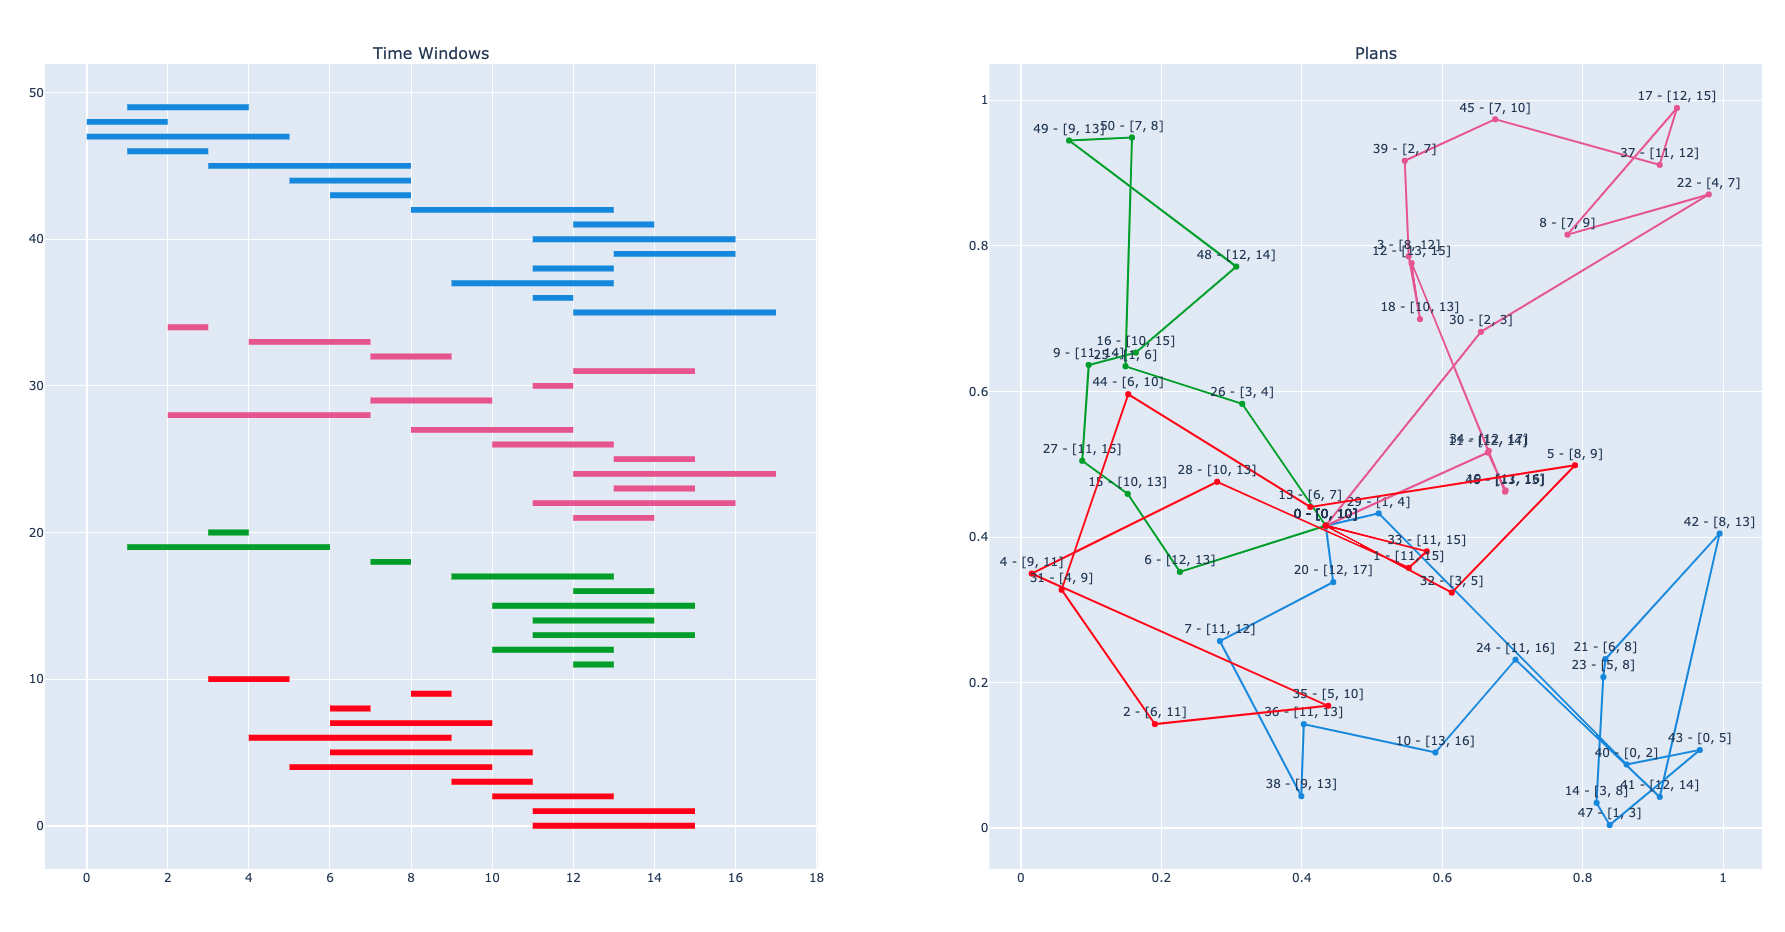
\includegraphics[width=1.0\textwidth]{resources/evaluation/sample-50.png}
    \caption{Properly distributed time windows across the vehicles.}
    \label{fig:nice-tw}
\end{figure}

\subsection{Balancing Plans}
In real-world solution of \gls{vrp}, we aim to balance the number of served customers across vehicles. It means the number of nodes in a given route is supposed to be uniformly distributed across all routes. However, we have noticed that the model was constantly adding additional routes of size one as illustrated on Figure \ref{fig:unbalanced}.

\begin{figure}[ht]
    \centering
    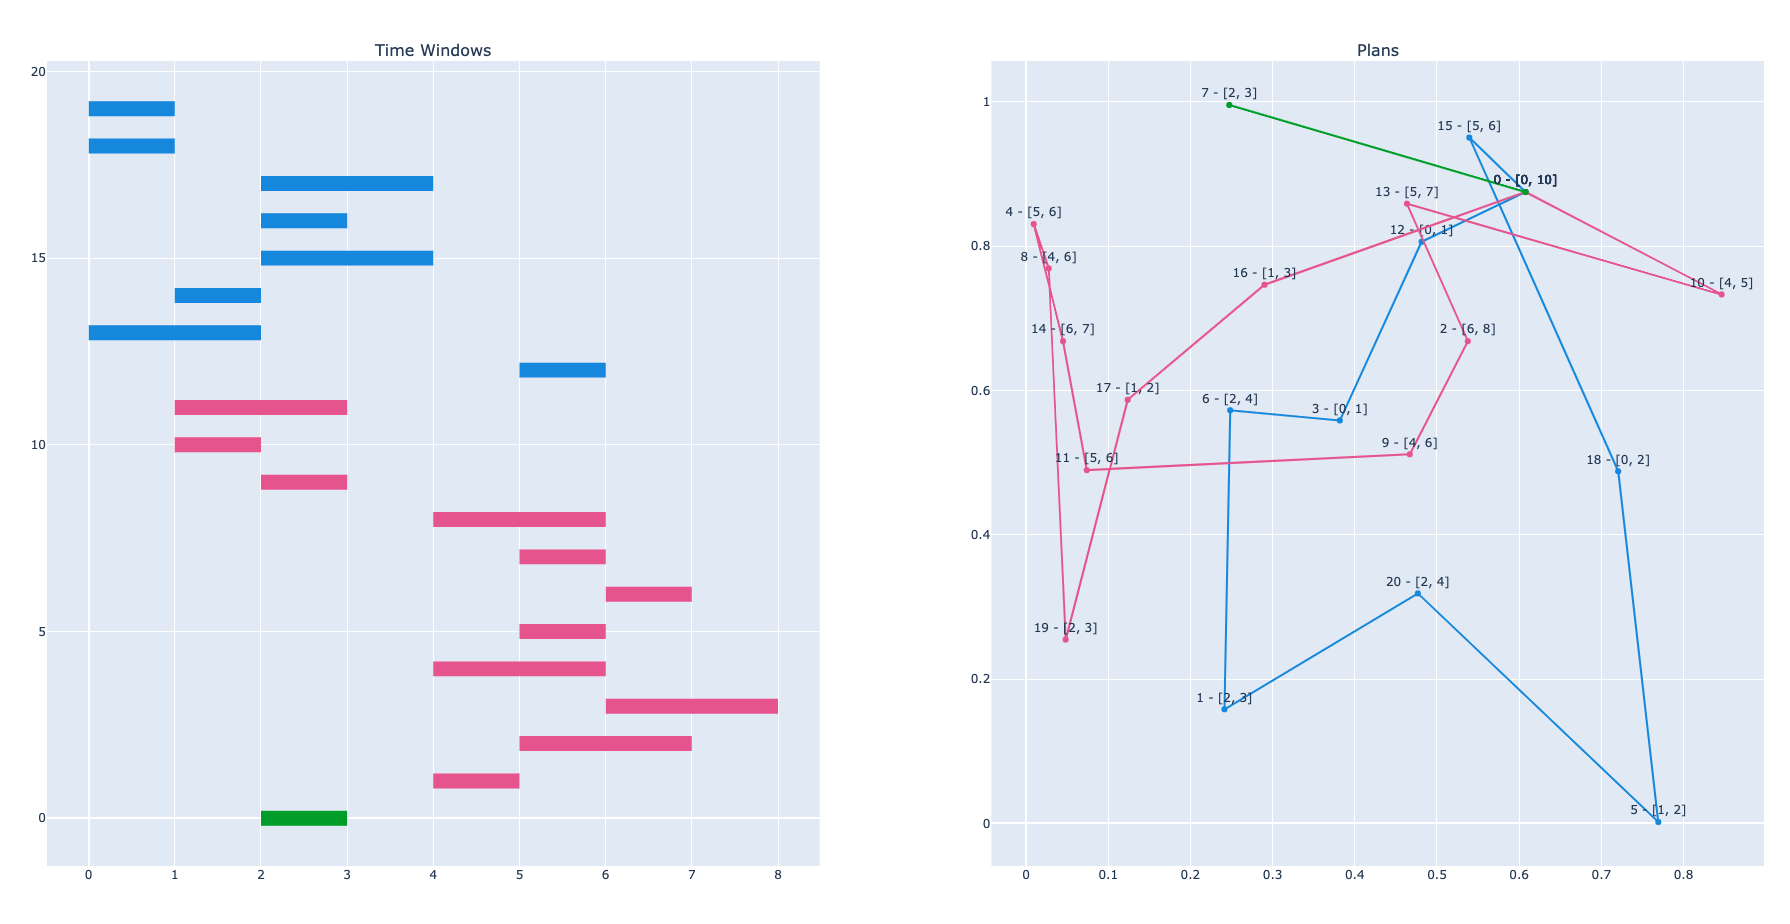
\includegraphics[width=1.0\textwidth]{resources/evaluation/unbalanced-plan.png}
    \caption{Unbalanced delivery plans.}
    \label{fig:unbalanced}
\end{figure}

Therefore, we have decided to penalize the delivery plans that are not balanced by including an unbalance penalty. We calculate the standard deviation of plans with the objective to be minimized using our cost function. This approach helped in creating balanced delivery plans.

\subsection{Generalization}
A great downside of this proposed model is its sensitivity to data input, which results in poor model generalization. If we introduce to a model a distribution of data which has not been seen before, it is not possible to predict sensible delivery plans and the model just serves each of the nodes by a single vehicle. This behavior is shown in Figure \ref{fig:model-breaks}. The model has even problems with generalization to different input data distributions in a single dataset.

\begin{figure}[ht]
    \centering
    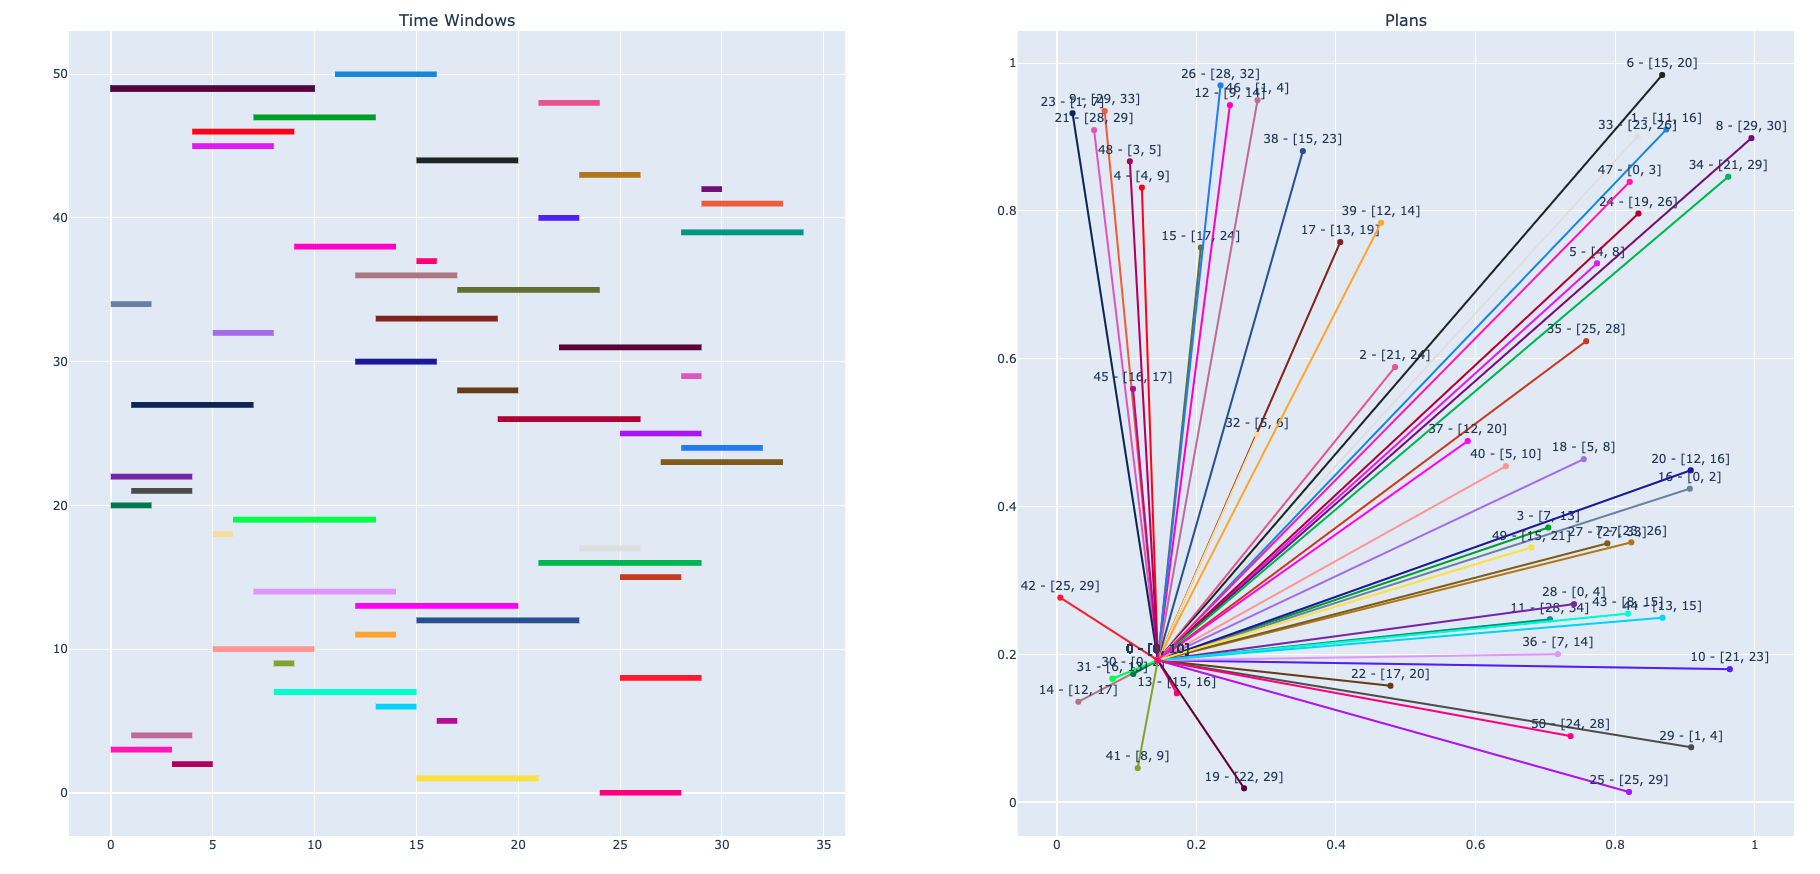
\includegraphics[width=1.0\textwidth]{resources/evaluation/data-sensitivity.png}
    \caption{If the model does not know how to solve the instance, it just sends each vehicle to serve one node.}
    \label{fig:model-breaks}
\end{figure}

Another model sensitivity is to the instance problem size. If the model is trained on the problem size of 20 nodes, the model performance is continuously degraded by a larger difference of the problem size on which it was trained on. We tried training the model on a dataset of different problem sizes, but the network was not effectively learning. The model has to be trained on a problem size with a minimal difference.

The solution is to train multiple models for each of the problem sizes and data distribution. However, this seems as a great obstacle in using this model in real-world environment and thus a new model with improved model generalization needs to be proposed by researches.

\subsection{Training Process}

The training process of such a network is very time consuming and with our limited available hardware, the \gls{vrptw} model for solving 50 nodes requires at least 5 days to be fully trained. Therefore, experimenting with a different values of network hyperparameters is not part of this thesis. We only focused on proving if even such a problem like \gls{vrptw} can be sub-optimally solved via \gls{ml}. We have used the same hyperparameters as Kool et al. \cite{attention-route} in their research.

During the training process, we have observed multiple values of the cost function \ref{vrptw-cost} to understand if the network was successfully learning to solve the problem.

\begin{figure}[ht]
    \centering
    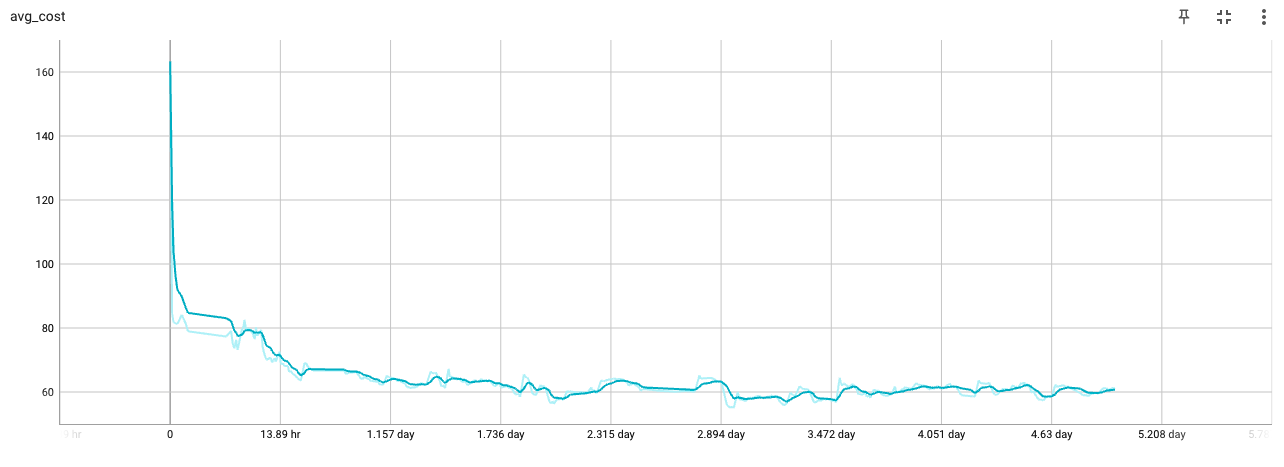
\includegraphics[width=0.75\textwidth]{resources/evaluation/avg-cost.png}
    \caption{Average cost (reward) per epoch on training data.}
    \label{fig:avg-cost}
\end{figure}

In Figure \ref{fig:avg-cost} we observe the average cost of the predicted solutions per epoch. It fairly quickly plateaued, but if we look at the average cost on the validation dataset \ref{fig:avg-cost-val}, the value was still decreasing. The model was still improving just on different parts of the cost function. 

\begin{figure}[ht]
    \centering
    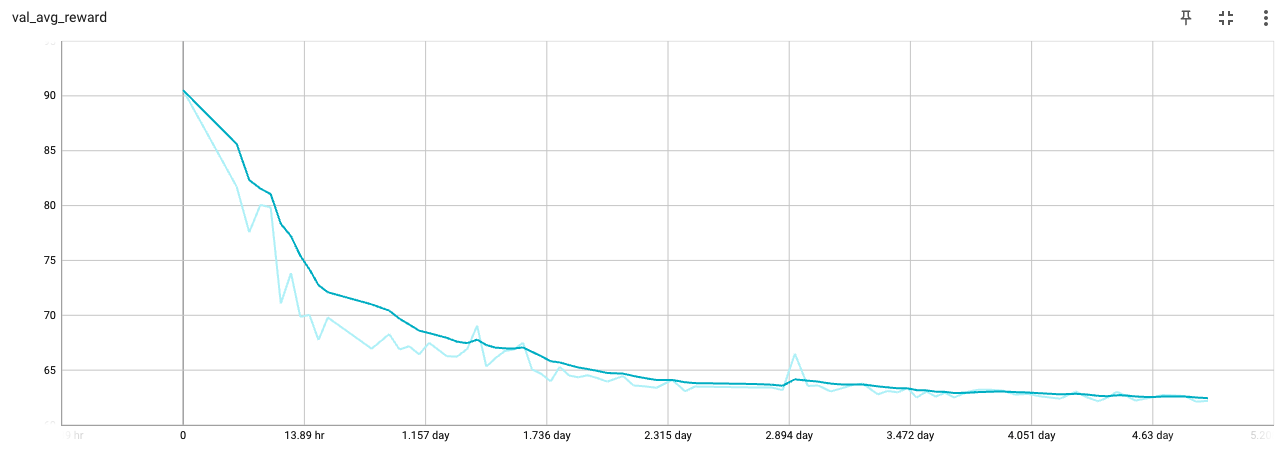
\includegraphics[width=0.75\textwidth]{resources/evaluation/val-avg-cost.png}
    \caption{Average cost (reward) per epoch on validation data.}
    \label{fig:avg-cost-val}
\end{figure}

If we would experiment with hyperparameter tuning, in this case, we could try to use the decaying learning rate which we assume would further more decreased the cost function.

\begin{figure}[ht]
    \centering
    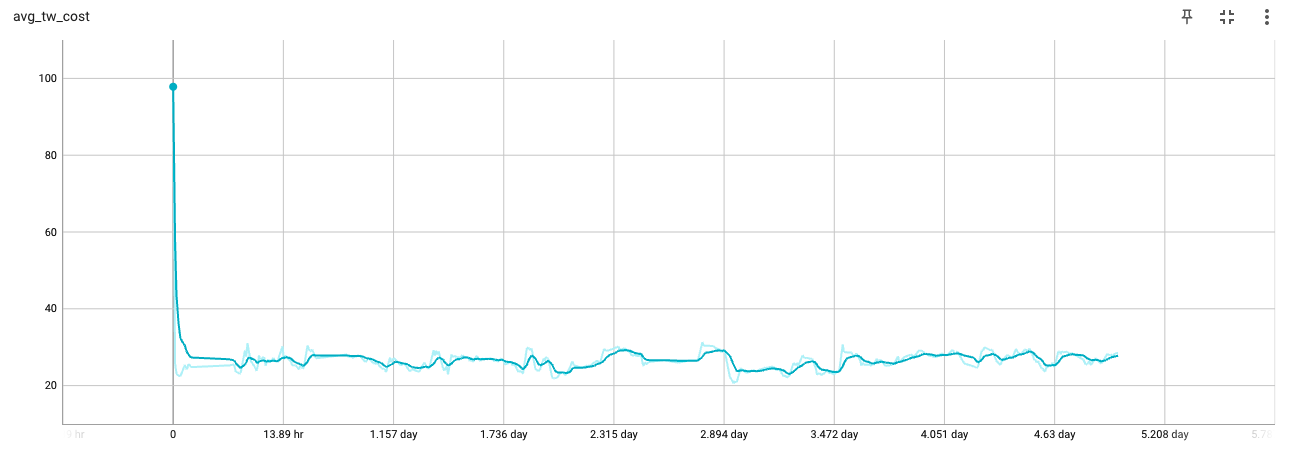
\includegraphics[width=0.75\textwidth]{resources/evaluation/avg-tw-cost.png}
    \caption{The average cost for time windows per epoch.}
    \label{fig:avg-cost-tw}
\end{figure}

In Figure \ref{fig:avg-cost-tw} we observe the average penalty for early and late arrivals of the predicted routes per epoch. The model quickly learns the policy strategy how to predict the next node to visit based on the time constraint. We assume that the model first learns the strategy for minimizing the time window based on the drastic drop of the time window cost function and then it learns to optimize the distance of routes. In Figure \ref{fig:avg-cost-distance} we observe the average total distance of predicted routes per epoch and the cost is constantly decreasing while the model learns to optimize the distance.

\begin{figure}[ht]
    \centering
    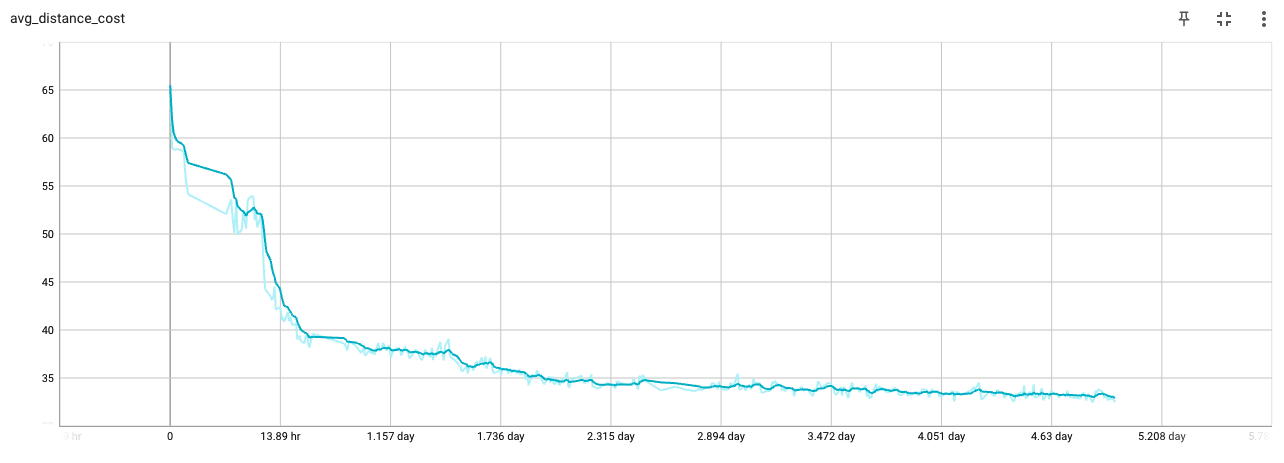
\includegraphics[width=0.75\textwidth]{resources/evaluation/avg-distance-cost.png}
    \caption{The average distance cost per epoch.}
    \label{fig:avg-cost-distance}
\end{figure}

In Figure \ref{fig:avg-cost-balance} is the last observed part of the cost function, the unbalance penalty, which is slowly decreasing while the model learns to distribute the nodes uniformly across the vehicles.

\begin{figure}[ht]
    \centering
    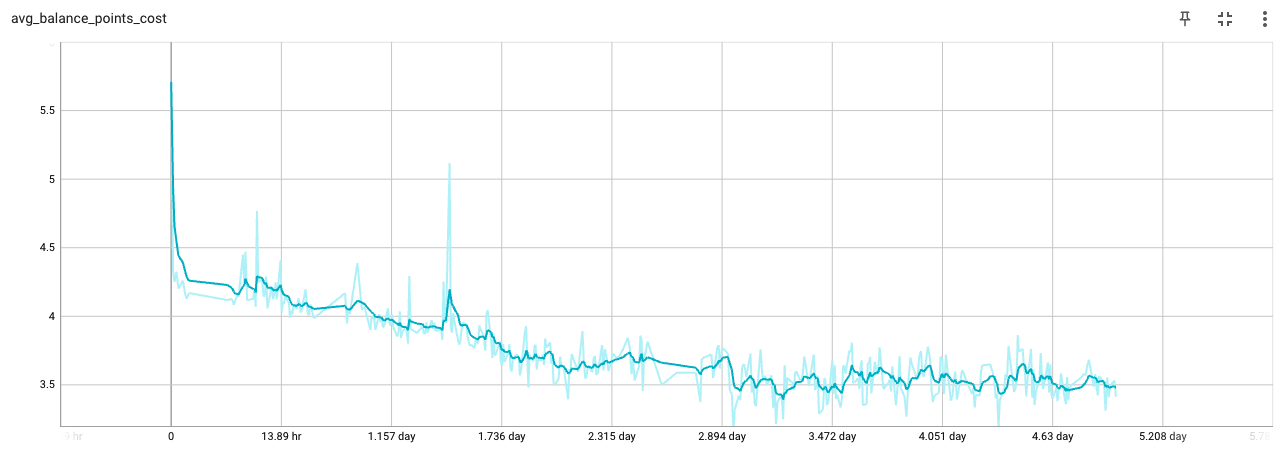
\includegraphics[width=0.75\textwidth]{resources/evaluation/avg-balance-cost.png}
    \caption{The average cost of balanced plans.}
    \label{fig:avg-cost-balance}
\end{figure}

The cost function is used as a reward function for \gls{rl}. It is important to note that the model can never achieve a value of the cost function which would converge to zero.
\newline

\section{Benchmarking}\label{benchmarking}
We know that our deep reinforcement learning model for sub-optimally solving \gls{vrptw} can predict a solution for \gls{vrptw} instances \ref{fig:sample-50}. However, to evaluate the model performance, we need to compare it with other reliable methods like constructive heuristics and metaheuristics.

The first benchmark is insertion heuristics \ref{insertion-heuristics} which produces a feasible solution in a matter of seconds. It is frequently used to generate an initial solution which is then optimized by a local search algorithm or population-based method. The second typical benchmark used in research papers is OR-Tools framework \ref{or-tools} and its is widely used for many optimization tasks. Lastly, the third benchmark combines insertion heuristics as an initial solution and OR-Tools planner as a metaheuristics.

\begin{table}[ht]
\centering
\resizebox{\textwidth}{!}{

\begin{tabular}{lrrrrr}
\toprule
{\textbf{Model}} & DistanceCost & DelayCost & EarlinessCost & ComputationTime & \textbf{AggCost} \\
{} &          Km &       min. &           min. &             sec &       \\
\midrule
\textbf{INSERTION\_HEURISTIC}    &           981 &          0 &            847 &                1 &    \textbf{1,193} \\
\textbf{RL\_AM\_PLANNER}          &           610 &         38 &            871 &                0.5 &      \textbf{847} \\
\textbf{OR\_TOOLS}               &           482 &          4 &            814 &              120 &      \textbf{687} \\
\textbf{OR\_TOOLS\_INSERTION}     &           488 &          1 &            798 &              121 &      \textbf{688} \\
\textbf{RL\_AM\_OR\_TOOLS\_PLANNER} &           482 &          4 &            814 &              120 &      \textbf{688} \\
\bottomrule
\end{tabular}

}
\caption{Benchmarking of VRPTW solvers for problem size of 20 nodes.}
\label{tab:result-20}
\end{table} 

In table \ref{tab:result-20} we may see the average cost of our implemented planners on 64 different \gls{vrptw} instances. 
The \textit{AggCost} is the same as being used in our model architecture \ref{vrptw-cost}.


\begin{table}[ht]
\centering
\resizebox{\textwidth}{!}{

\begin{tabular}{lrrrrr}
\toprule
{\textbf{Model}} & DistanceCost & DelayCost & EarlinessCost & ComputationTime & \textbf{AggCost} \\
{} &          Km &       min. &           min. &             sec &       \\

\midrule
\textbf{INSERTION\_HEURISTIC}    &         2,306 &          0 &          4,355 &               39 &    \textbf{3,395} \\
\textbf{RL\_AM\_PLANNER}          &         1,297 &        100 &          3,634 &                2 &    \textbf{2,255} \\
\textbf{OR\_TOOLS}               &           757 &        539 &          6,180 &              154 &    \textbf{2,571} \\
\textbf{OR\_TOOLS\_INSERTION}     &         2,007 &          3 &          3,967 &              192 &    \textbf{3,000} \\
\textbf{RL\_AM\_OR\_TOOLS\_PLANNER} &           759 &        537 &          6,161 &              156 &    \textbf{2,568} \\
\bottomrule
\end{tabular}


}
\caption{Benchmarking of VRPTW solvers for problem size of 50 nodes.}
\end{table} 


\begin{table}[ht]
\centering
\resizebox{\textwidth}{!}{

\begin{tabular}{lrrrrr}
\toprule
{\textbf{Model}} & DistanceCost & DelayCost & EarlinessCost & ComputationTime & \textbf{AggCost} \\
{} &          Km &       min. &           min. &             sec &       \\
\midrule
\textbf{INSERTION\_HEURISTIC}    &         4,654 &          0 &         17,548 &              750 &    \textbf{9,041} \\
\textbf{RL\_AM\_PLANNER}          &         5,852 &          1 &         15,805 &               16 &    \textbf{9,804} \\
\textbf{OR\_TOOLS}               &         1,034 &      2,885 &         23,719 &              199 &    \textbf{8,406} \\
\textbf{OR\_TOOLS\_INSERTION}     &         4,478 &          0 &         17,109 &              807 &    \textbf{8,755} \\
\textbf{RL\_AM\_OR\_TOOLS\_PLANNER} &         1,034 &      2,885 &         23,719 &              219 &    \textbf{8,406} \\
\bottomrule
\end{tabular}
}
\caption{Benchmarking of VRPTW solvers for problem size of 100 nodes.}
\end{table} 


